\chapter{Background}
\label{chapter:background}

\section{Ethereum Smart Contract}

\newpage
\section{MetaMask}
Metamask is a chrome extension for accessing Ethereum distributed application (DApp), this extension can enable web3 API in website so that users can interact with any Etehereum blockchain from Javascript~\cite{web3.js}, e.g., Mainnet, Testnet. It also creates identities by the user themself. The user of Metamask can create and manage their identities; moreover, Metamask provides an interface that user can perform a transaction to the connected blockchain.\par
Because the user securely  manages owned Ethereum account through MetaMask, the user can use their private key to sign a transaction or sign data to prove ownership of an account. Using this crypto wallet, the developers of decentralized applications can use their web3.js library to interact with MetaMask without maintaining Ethereum account of users and they can focus on designing and implementing functionality of smart contracts.\par
Regarding the architecture of Dapp, Figure~\ref{fig:architecture_of_dapp} shows that the web3.js libraries can enable user's browser to interact with blockchain so that users can read and write data from smart contracts, send transactions between accounts. 

\begin{figure}[hb]
    \centering
    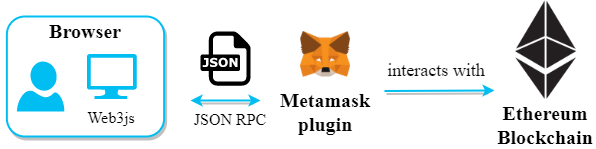
\includegraphics[height=!,width=1\linewidth,keepaspectratio=true]{figures/architecture_of_dapp.png}
    \caption{{\footnotesize Architecture of Dapp}}
    \label{fig:architecture_of_dapp}
\end{figure}

\section{ECDSA}
\newpage
\section{OAuth}

\section{Trust Service Provider (TSP)}

\section{Related work}
